\documentclass[../main.tex]{subfiles} 
\begin{document}
\chapter{Low-Level softwarebeveiliging}
\section{Introductie}
Een \emph{implementation-level software vulnerability} is een fout in een programma die door een aanvaller kan worden misbruikt.
In dit hoofdstuk hebben we het concreet over \emph{memory corruption vulnerabilies}.
Deze zwakheden zijn enkel relevant voor onveilige talen.
Dat zijn programmeertalen die niet controleren of programma's het geheugen correct gebruiken.
Hieronder staat een voorbeeld in ANSI c in listing \ref{l:intro}. Omdat er nergens de lengte van de input argumenten wordt nagekeken kan men in geheugen schrijven waar dat niet zou mogen.
Op die manier kan er arbitraire code worden uitgevoerd (een \emph{code injection attack}).
 
\lstinputlisting[style=cstyle, label=l:intro]{\codeSrc/intro_example.c}

\subsection{Achtergrond informatie}
Er kan op verschillende manieren geheugen gealloceerd worden in C:
\begin{description}
	\item[Automatisch] via locale variablen in functies.	
	\item[Statisch] via globale variablen.	
	\item[Dynamisch] via \lstinline[style=cstyle]{void *malloc(size_t size);} en \lstinline[style=cstyle]{new}.
\end{description}
De programmeur is verantwoordelijk voor dit geheugenbeheer van het alloceren tot het de-alloceren.
Figuur \ref{f:mem_lay} geeft de \emph{process memory layout} weer van een programma.
Hierbij groeit de heap naar boven (hogere adressen) en de stack naar onder (lagere adressen).
Indien de voorbeeld code \ref{l:intro} wordt ge\"exploiteerd bevind de geinjecteerde code zich in de Stack.
\begin{figure}
\centering
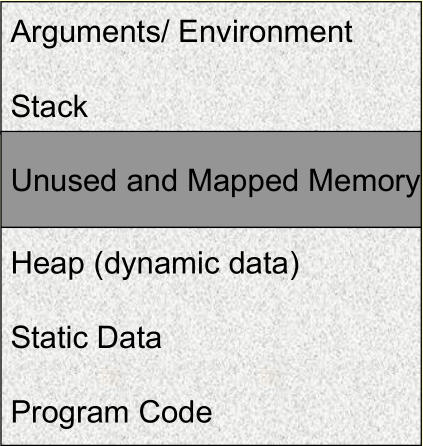
\includegraphics{\imageSrc/memory_layout.png}
\caption{Typische geheugen layout met bovenaan \textbf{hoge} adressen.}
\label{f:mem_lay}
\end{figure}


\section{Aanvals voorbeelden}
\subsection{Stack-based buffer overflow}
\subsection{Heap-based buffer overflow}
\subsection{Return-to-libc attacks}
\subsection{Data-only attacks}
\section{Verdedigings voorbeelden}
\subsection{Stack canaries}
\subsection{Non-executable data}
\subsection{Control-flow integrity}
\subsection{Layout randomization}
\section{Conclusie}
\end{document}
